\documentclass{whutmod}
\usepackage{metalogo}
\usepackage{float}
\usepackage{subfigure} 
\usepackage{url}
\usepackage{booktabs}
\bibliographystyle{unsrt}
\team{23}
\membera{刘子川}
\joba{编程}
\memberb{程宇}
\jobb{建模}
\memberc{陈荣兴}
\jobc{建模}
\hypersetup{
	colorlinks=true,
	linkcolor=black
}

\title{基于因子分析与灰色关联分析对武汉市人才吸引力的量化评价}
\tihao{4} 

\begin{document}

	%\maketitle
	
	\begin{abstract}

城市的发展对人才的吸引力两者之间是相互联系与制约的,因此需要政府决策与措施影响,使城市增强对人才的吸引力。本文结合武汉的发展特点,利用\textbf{爬取}后的数据较全面的选择合适的指标进,通过\textbf{因子分析}的方法为武汉市不同年份人才吸引力打分;再对人才进行产业类别分类,通过\textbf{灰色关联分析}筛选出合适的因子后再横向比较各城市综合得分,并结合当地人才政策评价对人才吸引力的水平提出合理化建议。
~\\%~\\为换行

针对问题一,通过\textbf{因子分析模型}分析武汉2013—2017年相关数据,对武汉各年的人才吸引力进行\textbf{量化打分}。本组首先根据题目要求和以往人才吸引要素研究,确立要素框架并\textbf{爬取}合适的人才吸引力因素。在标准化数据通过\textbf{KMO检验}后,利用SPSS对各个因素进行\textbf{主成分分析}以确定公因子数目,求解旋转后因子荷载矩阵并对公因子命名,计算武汉各年人才吸引力综合得分。综合得分结果为\textbf{-77.99、-30.08、-11.90、42.35、77.63}。综合得分表明武汉2013—2017人才吸引力逐年上升,且2015—2016年上升幅度最大,与城市实际发展情况相符合。
~\\

针对问题二,本文在问题一模型的基础上进行改进,将人才分为第一、第二和第三产业人才并用\textbf{灰色关联分析}筛选出每类人才相应的人才吸引力因素。然后将筛选后的数据用SPSS进行\textbf{因子分析}得到成都、天津、西安、南京和武汉2013—2017年的三类人才吸引力因子分析模型,并计算每个城市各年针对三类人才的人才吸引力\textbf{综合得分}。横向比较各个城市的综合得分,相较与其他城市,武汉市近几年对第二、三产业人才的吸引力有较高水平,相对于西安和成都,武汉市具有较强的人才吸引力,符合地区的经济发展特点。
~\\

针对问题三,基于问题一中的武汉市人才吸引力评价模型以及人才政策对人才吸引力的量化评价,并结合问题二中武汉相较于其他四个同类城市在人才吸引力上的优势与不足,给武汉市人力资源管理部门的领导写一篇建议报告。
~\\

本文中所提到的模型优点主要有两点:一、选取的指标从多维度、全方面考虑,收集的数据真实可靠;二、利用灰色关联度筛选出三类人才的人才吸引力要素,相较于人工选取指标具有客观性、严谨性。
  
\keywords{因子分析模型\quad  主成分分析\quad  灰色关联分析\quad 数据库爬虫\quad }
		
	\end{abstract}
	
	%目录
	\tableofcontents
	\newpage	%换页符
	
	\section{问题重述}	
	\subsection{问题背景}
    植物的种类繁多,要了解和掌握如此多的植物,必须进行一个科学的分类。人们常常根据植物的用途,或根据植物的一个或几个明显的形态进行分类,植物的识别与分类对于区分植物种类,探索植物间的亲缘关系,阐明植物系统的进化规律具有重要的意义。因此植物分类学是植物科学甚至整个生命科学的基础学科。目前对于树叶识别与分类主要由人完成,但是树叶种类庞大,依赖人工地进行树叶识别与分类是不现实的。所以树叶的研究对于植物总体的研究能提供很大的帮助。
    
    从树叶的各个方面,纹理,硬度,离心率等方面都可作为主要方向研究,现对树叶的研究主要通过采集树叶图形,利用数字图像处理来对树叶进行分类识别,这种方法只停留在处理形态特征,有很大的局限性,忽略了树叶的生理特征和其他特征,所以研究方法来综合处理树叶平面图像特征,形态特征和生理特征很有必要性。
    
    

	\subsection{问题提出}
    围绕植物分类进行树叶识别与分类,以树叶二值化图片为依据,依次提出以下问题:
		 
	\begin{itemize}
	\item [(1)] 结合附件中的二值化的图片数据,建立合适的图片数据提取方案, 量化处理图片数据,并具体分析说明所提取数据信息的量化指标体系。
	\item [(2)] 基于问题一中提取的数据信息,建立合适的数学模型由数据出发判断叶子的种类,研究判别分类的核心指标,并估计出模型的性能以及核心指标对模型判别性能的影响。
	\item [(3)] 基于二值化图片数据,结合附件中叶子纹理的数据信息,对原有模型进行改进,并对新旧模型进行比较分析。
	\end{itemize}
	
	\section{模型假设}
	\begin{itemize}
		\item [(1)] 假设相同的行业在不同的城市里吸引力影响因素相同,每个行业在不同城市里的发展模式近似相同。
		\item [(2)] 人才会考虑未来一段时间内自身对于发展前景、收入、环境的需求的变化。
		\item [(3)] 政策对人才吸引力的影响转换成三个影响因素——地方财政支出与收入和固定资产投资总额。
		\item [(4)] 人才的迁移是在追求效用最大化,人才的行为仅受到城市因子的影响,忽略人的非理性行为。
	\end{itemize}
	
	
	\section{符号说明}
%	每行都有线的表
%	\begin{center}
%		\begin{tabular}{cc}
%			\hline
%			\makebox[0.3\textwidth][c]{符号}	&  \makebox[0.4\textwidth][c]{意义} \\ \hline
%			$C_{0}$	    &  污染源初始浓度 \\ \hline
%			$C(x,t)$	    &  污染浓度随时空变化 \\ \hline
%			$u_{x}$	    &  江河平均纵向流速 \\ \hline
%			$E_{x}$  &  铊在江河纵向弥散系数\\ \hline
%		$p$   &  面污染物纵向距离\\ \hline
%			$K_{c}$	    & 污染物降解系数  \\ \hline
%		    $a$	& 污染超标系数 \\ \hline
%		     $x$	& 距污染源的一维距离 \\ \hline
%		      $t$	& 距污染发生后的时间 \\ \hline
%		       $V_{A}$	& 溶液摩尔体积 \\ \hline
%		      $M_{B}$	& 江水的摩尔质量 \\ \hline
%		     $\mu_{B}$	& 溶剂的粘度 \\ \hline		      
%		\end{tabular}
%	\end{center}

%三线表
	\begin{table}[H]
	\label{biao} \centering
		\begin{tabular}{cc}
			\toprule[1.5pt]
			\multicolumn{1}{m{5cm}}{\centering 符号} & \multicolumn{1}{m{5cm}}{\centering 说明} \\
			\midrule[1pt]
			$F$	 &  城市各年人才吸引力综合得分  \\ 
			$F_{1}$ &  工业发展与薪酬因子 \\ 
			$F_{2}$	 &  医疗卫生环境因子 \\ 
			$F_{3}$  &  经济贸易因子 \\ 
			$F_{4}$  &  拥挤程度因子 \\ 
			$X$  &  原始指标 \\ 
			$\overline{X}$  &  指标平均值 \\ 
			$\widetilde{X}$  &  同向化指标 \\ 
	     	$\delta_{X}$  &  指标标准差 \\ 
	     	$Z$  & 标准化指标 \\ 
	     	$R$  & 相关系数矩阵 \\ 
	     	$\lambda_{p}$  & 相关系数矩阵特征值 \\ 
	     	$\eta _ {p}$  & 标准正交化特征向量 \\ 
	     	$\Lambda$ & 因子载荷矩阵 \\ 
	     	$\sigma_{i}$ & 方差 \\
	     	$\alpha_{i j}$ & 载荷因子 \\
	     	$k$ & 两极最小差 \\
	     	$K$ & 两极最大差 \\
	     	$\Delta _{i}(t)$ & 特征序列与因素序列的序列差 \\
			\bottomrule[1.5pt]
		\end{tabular}
	\end{table}

	\section{问题一模型的建立与求解}
	\subsection{问题的描述与分析}

	针对问题一,本题要求建立合适方案提取二值化图片中的数据,并对所提取数据的量化指标进行分析说明。本组通过解析几何计算和时间序列展开,将目标图像转化成两个特征向量。本组根据题目要求和近年的图像识别研究,确定了针对二值化图像的两个重点识别因素——轮廓特征因素和边缘特征因素。针对轮廓特征因素,首先利用matlab做解析几何运算,计算与图像轮廓有关的特征量,并将计算结果作为元素,组成轮廓特征向量。针对边缘特征因素,首先将图像边缘通过极化投影展开为时间序列,计算每支时间序列的特征量,并将计算结果作为元素,组成边缘特征向量。最后合并两个向量得到总体特征向量。
	    \subsection{模型的建立}
	    \subsubsection{图像基本参数定义}
		定义$I$表示目标树叶所对应的图像,$\partial I$表示图像边界,$D(I)$表示图像最小外接圆直径,$d(I)$表示图像最大内切圆半径,$A(I)$表示研究对象面积,$L(\partial I)$表示研究对象的轮廓线长度,$H(I)$表示研究对象的凸包域,$C(I)$为图像几何中心坐标,运算符$d(.)$代表欧式距离。
	    \subsubsection{轮廓特征因素}
		定义轮廓特征向量为$ID1_{1}=[id_{1},id_{2},\cdots,id_{n}](n=6)$其中$id_{k}(k=1,2,\cdots,6)$为二值化矩阵的轮廓特征,其具体计算公式如下:
		\begin{itemize}	
		\item [$id_{1}$]长宽比(Aspect Ratio):
		定义$X_{I}$为图像最上方非零行与最下方非零行的行数差(长),$Y_{I}$为图像最左方非零列与最右方非零列的列数差(宽),长宽比$id_{1}=X_{I}/Y_{I}$。
		
		\item [$id_{2}$]离心率(Eccentricity): 
		定义$E(I)$是与研究图像具有相同的二阶矩的椭圆,$a$和$b$分别为$E(I)$对应的长轴与短轴,离心率$id_{2}=\sqrt{1-(\frac{b}{a})^{2}}$,变化范围为(0,1)。
		
		\item[$id_{3}$]密实度(Solidity):
		实密度$id_{3}=\frac{ A }{A(H(I))}$。其反映研究对象的仿射特征,即研究对象区域的固靠性程度。
		
		\item [$id_{4}$]等周因子(Isoperimetric Factor):
		等周因子$id_{4}=\frac{4\pi \cdot  A}{L(\partial I)^{2}}$ ,其变化范围为(0,1),描述目标树叶轮廓规整度,叶子边缘越规则,其值越接近于最大值1。
		
		\item [$id_{5}$]伸长率(Elongation): 
		伸长率$id_{5}=1-\frac{2d_{I}}{D(I)}$,变化范围为(0,1),树叶越趋于圆形,相应的伸长率越小,比率$\frac{2d_{max}}{D(I)}$ 其描述目标树叶轮廓向外伸展的趋势。
		
		\item[$id_{6}$]最大压痕深度(MaximalIndentationDepth):
		定义$C_{H(I)}$为研究对象凸型区域的几何中心,$L(\partial I)$表示为$H(I)$的轮廓线长度,$\forall X\in H(I)$和$\forall Y\in \partial I$,计算距离$d(X,C_{H(I)})$和$d(Y,C_{H(I)})$。定义函数$\frac{ d(X,C_{H(I)})- d(Y,C_{H(I)})}{L(H(I))}$,该函数的最大值即最大压痕深度$id_{6}$。
	\end{itemize}
		
		\subsubsection{边缘特征因素}
		为得到研究对象的边缘特征,首先以$C(I)$为坐标原点建立笛卡尔坐标系,对于曲线$\partial I$上任意一点$P$可以在该坐标系下表示为$P(x_{p},y_{p})$,将其投影至以$C(I)$为极点的极坐标系得${P}'(r_{p},\theta _{p})$,其中:
		\begin{gather}
		r_{p}=d(P(x_{p},y_{p}).C(I))
		\end{gather}
		\begin{gather}
		\theta _{p}=y_{p}/x_{p},
		\end{gather}
		(图1)
		通过将点集${{P}'(r_{p},\theta _{p})}$降维可得到时间序列$arrays({P}')$。将arrays滤波处理后,计算每支时间序列上的极大值点数$id_{7}$,极小值点数$id_{8}$。得到边缘特征向量$ID2=[id_{7},id_{8}]$,合并轮廓特征向量与边缘特征向量得:
		\begin{gather}
		ID=[ID1,ID2]
		\end{gather}
	     其中ID为总体特征向量。
	      \subsection{模型的求解}
	      首先使用matlab围绕regionprops函数对研究对象进行解析几何计算,用遍历式算法逐一算出研究对象长宽比、离心率、实密度、等周因子、伸长率和最大压痕深度,得到轮廓特征向量(见代码?)。再将图片通过numpy工具箱标准正立化,以其几何中心为极点将其边缘坐标转换为极坐标,然后使用ndarrays函数将所得极坐标降维展开成时间序列,搜寻滤波后时间序列的极点数得到边缘特征向量。
	

	
	\section{问题二模型的建立与求解}
	\subsection{问题的描述与分析}
	问题二要求针对所提取数据信息,建立数学模型判别叶子的种类并研究其核心指标。本组通过问题一中所提取的$11$维度的特征,采用$Keras$工具库搭建深度神经网络(DNN)解决树叶多分类问题,并输出各维度特征的权重作为指标贡献率。DNN神经网络采用BP算法基于梯度信息来调整连接权值,因而初始权值和阈值选取的随机性会导致网络稳定性差。为克服此缺点,引入收敛速度快、全局搜索能力强的PSO算法来优化DNN网络的连接权值和阈值,建立一种新的$PSO-DNN$网络模型实现对树叶分类。当考虑到步长等参数的选取时,使用网格搜索的方式对参数进行优化,其流程图如下:
		
	\begin{figure}[H]
	\centering
	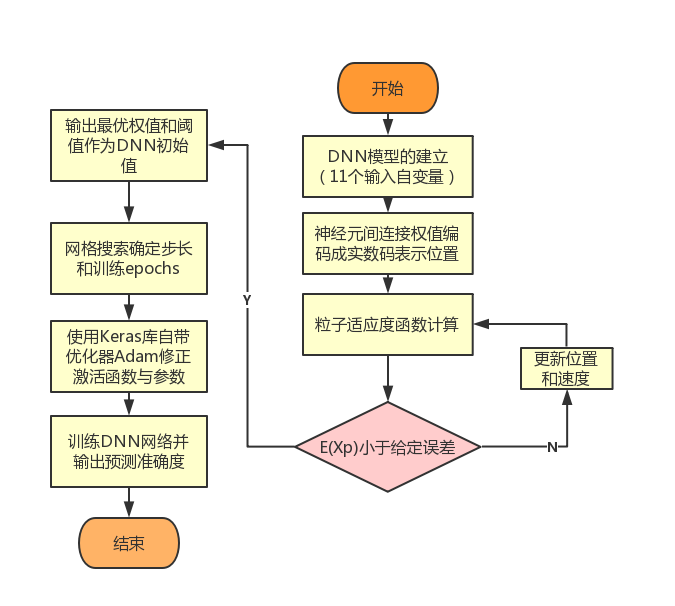
\includegraphics[width=\textwidth]{figures/21.png}
	\caption{PSO算法优化DNN网络流程图}\label{2222}
	\end{figure}


	\subsection{模型的建立与求解}
	
	\subsubsection{DNN网络搭建}
	DNN的正向传播主要依靠众多神经元的计算来完成的,此处设计的网络结构如图~\ref{dnn}~所示,工作过程中可以用下式来表示:
			\begin{gather}
{u_{k}=\sum_{i=1} w_{k i} x_{i}} \\ {y_{k}=f\left(u_{k}-b_{k}\right)}
	\end{gather}
	其中:$x_{i}$表示第 i 个输入; $w_{ki}$表示与第 i 输入量相 连的权值; $u_{k}$表示所有输入的加权和; $b_{k}$为神经 元阈值;$ f$ 为激活函数; $y_{k}$ 为神经网络的输出。
	
	激活函数的种类有很多,如 $sigmoid$, $tanh$ 及$ Relu$,本文应用的是 $ReLU$作为激活函数搭建两层隐层,如式~\ref{shiw}~所示:
	\begin{gather}\label{shiw}
		\begin{array}{c}{f_{\text {Relu}}=\max (0, z)}\\
		\frac{d}{d z} f_{R e L U}=\left\{\begin{array}{ll}{1,} & {z>0} \\ {0,} & {z \leqslant 0}\end{array}\right.
		\end{array}
	\end{gather}
	
	网络的输出层使用$ softmax $函数作分类器, 式~\ref{shiq}~为第 i 个神经的输出:
	\begin{gather}\label{shiq}
		f_{\text {softinax }}=\mathrm{e}^{i} / \sum_{j} \mathrm{e}^{j}
	\end{gather}
	
		\begin{figure}[H]
		\centering
		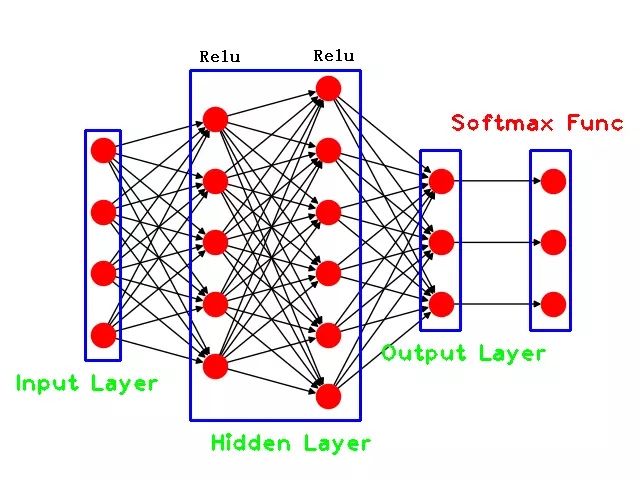
\includegraphics[width=\textwidth]{figures/sss.png}
		\caption{人工搭建DNN结构示意图}\label{dnn}
	\end{figure}
	
	
	\subsubsection{PSO-DNN网络初始值确定}
	算法的具体实现步骤如下:
	\begin{itemize}
		\item [(1)]将DNN网络结构中所有神经元间的连接权值和各个神经元的阈值编码成实数码串表示的个体作为PSO算法要寻优的位置向量。
		\item [(2)]在编码空间中随机生成一定数目的个体组成种群,其不同个体代表神经网络不同权值。
		\item [(3)]DNN
	\end{itemize}
	
	\subsubsection{分类型人才吸引力分析}
	将归类后所得的影响第一产业人才吸引力的$10$个影响因素在五个城市中2013—2017年的数据,使用SPSS进行因子分析,按照累积贡献率的原则提取公因子,以综合性指标来相对全面的反映出全体因子对第一产业人才吸引力的影响情况。按照主因子的提取原则,通过碎石图可看出可以用$3$个主因子来描述此$10$个因子的影响;再通过旋转后因子贡献率计算所得的城市各因子得分得到各城市每年的第一产业人才吸引力综合得分。其计算公式如下:
	\begin{gather}
	\mathrm { F } = \left( 48.328 \mathrm { F } _ { 1 } + 28.667 \mathrm { F } _ { 2 } + 12.283 \mathrm { F } _ { 3 } \right) / 89.277
	%(附结果计算公式)
	\end{gather}
	将得到的五个城市2013—2017年的综合得分绘制为折线图的到图~\ref{11}~如下所示:
	\begin{figure}[H]
		\centering
		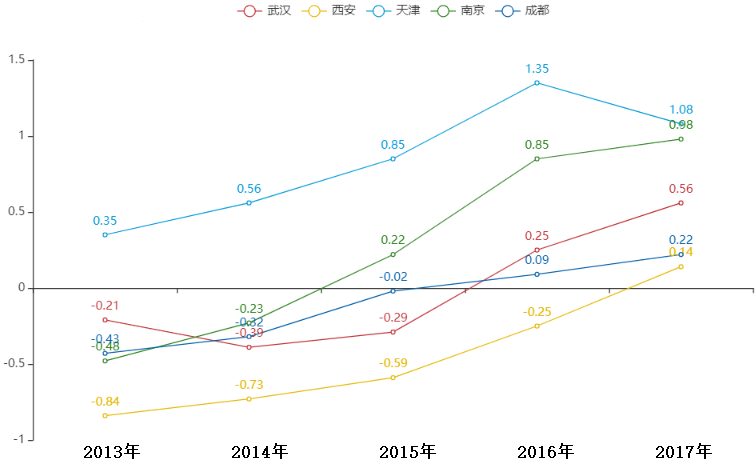
\includegraphics[width=.9\textwidth]{figures/11.png}
		\caption{第一产业人才吸引力综合得分折线图}\label{11}
	\end{figure} 
	同理将归类后所得的影响第二产业人才吸引力的$10$个影响因素使用SPSS进行因子分析,得到第二产业人才吸引力综合得分计算公式:
	\begin{gather}
	\mathrm { F } = \left( 27.594 \mathrm { F } _ { 1 } + 26.960 \mathrm { F } _ { 2 } + 16.609 \mathrm { F } _ { 3 } + 16.356 \mathrm { F } _ { 4 } \right) / 87.519
	%(附结果计算公式)
	\end{gather}
	第二产业人才吸引力综合得分折线图:
	\begin{figure}[H]
		\centering
		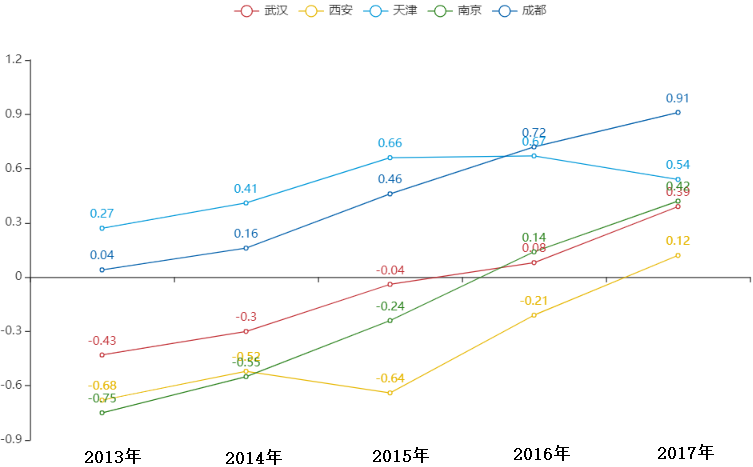
\includegraphics[width=.9\textwidth]{figures/22.png}
		\caption{第二产业人才吸引力综合得分折线图}\label{22}
	\end{figure}
	
	同理将归类后所得的影响第三产业人才吸引力的$10$个影响因素使用SPSS进行因子分析,得到第二产业人才吸引力综合得分计算公式:
	\begin{gather}
	\mathrm { F } = \left( 37.063 \mathrm { F } _ { 1 } + 25.130 \mathrm { F } _ { 2 } + 11.972 \mathrm { F } _ { 3 } + 10.477 \mathrm { F } _ { 4 } \right) / 84.642
	%(附结果计算公式)
	\end{gather}

	第三产业人才吸引力综合得分折线图:
		\begin{figure}[H]
		\centering
		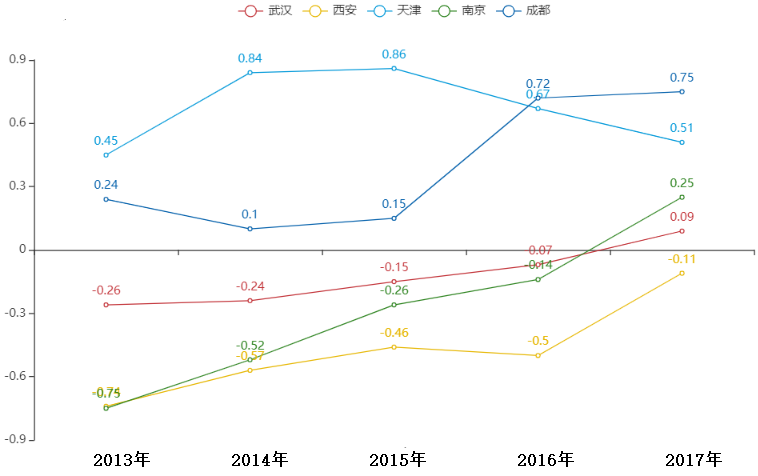
\includegraphics[width=\textwidth]{figures/33.png}
		\caption{第三产业人才吸引力综合得分折线图}\label{33}
	\end{figure}


	\subsection{结果分析}
	由图表可以看出,武汉市的人才吸引力水平近几年有较高的水平,尤其是对第二、三产业人才的吸引力表现出逐年增加趋势和较高水平,相对于西安和成都而言,武汉市具有较强的人才吸引力,十分符合地区的经
	济发展特点。而天津作为老牌北方直辖市,近年发展速度相比略显缓慢,导致其相应人才吸引力也有所下滑。
	
	但是,武汉在发展中也存在一些不足。特别是工业发展与薪酬因子处于人才吸引主导地位,而环境方面的因素尚未
	完全建立;优质教育与医疗资源分
	配不均、生活成本高、高校科研机构偏少等因素限制良好人才环境
	构建等。
	
	提高武汉市的人才吸引力水平,提出以下几点建议:
\begin{itemize}
	\item [(1)] 大力发展地方生产总值,为经济社会发展打下坚实的基础。
	\item [(2)]主要行业是加快人
	才发展的主导力量。建立较为高效的人才市场,通过各行业市场
	机制,人才较为充分地实现了自身价值,也为武汉的人才持续发展创
	造了良好条件。
	\item [(3)]注重整合空间结构全面发展,引导各大区块均衡协调稳步发展,
	建设全面型社会,注重生态建设,贯彻落实以人为本的科学发展理
	念。
	\item [(4)]加大营商环境改革力度,营
	造更加开放的贸易投资环境,营造综合成本适宜的产业发展环境,
	营造更加高效透明的政务环境。
	\item [(5)]政府不断完善就业服务政策,出台大量相关文件,高度重视高
	校毕业生的就业情况。
\end{itemize}

	\section{写给武汉市人力资源部门的建议报告}
	
	\section{模型的评价}
	\subsection{模型的优点}
	\begin{itemize}
		\item [(1)] 从国家统计数据库、武汉市统计年鉴和其他同类城市的统计年鉴中爬取大量数据,并挑选符合实际的33个指标与最近五年的数据进行评价。其吸引人才指标从多维度、全方面的考虑,具备科学性、客观性。
		\item [(2)]针对具体人才根据相应产业进行分类。相较于现有城市人才吸引力水平评价模型,我们采用了灰色关联分析法,对三种人才类别分析计算出与指标的相关系数,求出不同人才对33种影响因素的的偏好程度,选出前十个合适的指标进行综合打分。
	\end{itemize}

	
	\subsection{模型的缺点}
    未能具体地量化政府政策对人口吸引力的影响,只选取了地方财政收入、支出,固定资产投资总额三个影响因素作为政策影响的指标,与现实情况出现一定偏差,存在一定的局限性。

    
    
	\newpage	%换页符
	%%参考文献
	%\begin{thebibliography}{9}%宽度9
	% \setlength{\itemsep}{-2mm}
	\nocite{*}		%排版未引用的参考文献
\bibliography{wenxian.bib}
	%参考文献添加到wenxian.bib里,再引用
	
	\newpage
	%附录
	\appendix %%附录
\section{代码}
\subsection{数据预处理--python源代码}
\begin{lstlisting}[language=python]%这里修改语言
import pandas as pd
from sklearn.preprocessing import StandardScaler
from sklearn.decomposition import PCA
from factor_analyzer import FactorAnalyzer

#导入数据
df = pd.read_excel("wut.xls")
# print(df.head(5))

#转置
df = pd.DataFrame(df.values.T, index=df.columns, columns=df.index)
# print(df['商品房平均销售价格(元/平方米)'])

数据正向处理
df['商品房平均销售价格(元/平方米)'] = -(df['商品房平均销售价格(元/平方米)']-sum(df['商品房平均销售价格(元/平方米)'])/5)
df['工业废水排放量(万吨)'] = -(df['工业废水排放量(万吨)']-sum(df['工业废水排放量(万吨)'])/5)
df['工业二氧化硫排放量(吨)'] = -(df['工业二氧化硫排放量(吨)']-sum(df['工业二氧化硫排放量(吨)'])/5)
print(df['商品房平均销售价格(元/平方米)'])
print(df.head(5))
df.to_excel("武汉.xls")

#数据标准化
df = StandardScaler().fit_transform(df)
# print(df)
df=pd.DataFrame(df)
df.to_excel("武汉.xls")
#
#主成分分析
pca = PCA(n_components=4)
newX = pca.fit_transform(df)
print(newX)

#返回所保留的n个成分各自的方差百分比
print("它代表降维后的各主成分的方差值占总方差值的比例,这个比例越大,则越是重要的主成分")
print(pca.explained_variance_ratio_)
print("它代表降维后的各主成分的方差值,方差值越大,则说明越是重要的主成分")
print(pca.explained_variance_)

\end{lstlisting}


\end{document}